\chapter{Nově navržený systém}
\label{Nově navržený systém}
%V této kapitole se budem zabívat nově navrženým systémem, jejíma komponentama a... 
Nově navržený systém se skládá z databáze a 5 hlavních komponent navzájem propojených: mikrokontrolér, váha, čtečka čárového kódu, displej a klávesnice. Dále je možnost připojit systém k počítači pro správu databáze a tisk dat. 

\section{Postup měření}%/Princip/funkcionalita
Pro evidenci zůstatkového objemu jedné láhve je nutné naskenovat její čárový kód pomocí čtečky čárových kódů a zvážit ji. Mikrokontroler na základě získaného EAN vybere z databáze patřičná data, viz kapitola č. \ref{databaze} a přepočítá hmotnost na objem. V případě, že by čárový kód nebyl čitelný, je možné ho zadat ručně do systému prostřednictvím klávesnice. Veškeré důležité informace včetně zbytkového objemu se zobrazí na displeji. Pro výpis všech naměřených dat je možné systém připojit k počítači a nechat si je vytisknout do formátu .xlsx pomocí navržené desktopové aplikace. Tato aplikace slouží i ke správě databáze.
%Do budoucna k měřicimu systému bude vyvíjena aplikace, 

\section{Blokové schéma}
%FOTO
%Výpočetní jednotka Raspberry pi pracuje s databázi dat jednotlivých destilátů. V první řadě je nutné tuhle databází vytvořit a implementovat prostřednictvím desktopové aplikace. 
\begin{figure}[!h]
    \begin{center}
        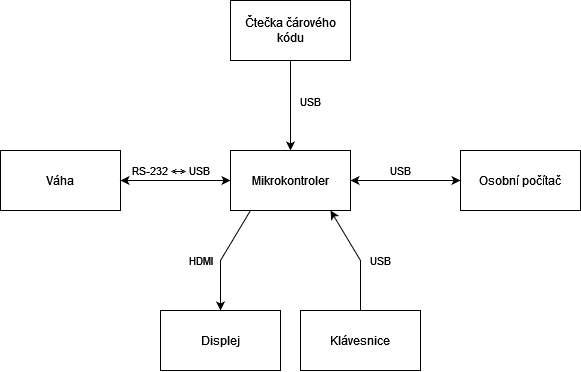
\includegraphics[scale=0.7]{obrazky/Blokové schéma.png}
    \end{center}
    \label{blokove_schema}
    \caption{Blokové schéma nově navrženého systému}
\end{figure}

\section{Databáze}
\label{databaze}
%Celý systém je závislý na datech, které nesou informace o názvu destilátu
Aby bylo možné přepočítat hmotnost na objem je nutné znát předem hmotnost prázdné a plné láhve a její maximální objem. Postup výpočtu je zmíněn v kapitole č. \ref{odkazos}. Tyto data jsou uloženy v databázi včetně informací jako jsou: název destilátu, EAN kód, maximální objem, nebo adresa k obrázku daného produktu.
%K datům se přistupuje pomocí EAN kódu nebo názvem destilátu zadaný klávesnicí.

%Některé destiláty, mají na svém hrdle nalévač místo vršku, který mění hmotnost láhve. Aby naš systém byl časově efektivní, tak implementujeme druhou databázi 

Některé destiláty mají na svém hrdle nalévátko (obrázek č. \ref{nalevačos}) místo víčka, který mění hmotnost láhve. V takovém případě bychom museli nalévač nahradit víčkem, aby hmotnost láhve odpovídala předpisu funkce, což je časově neefektivní. Místo toho byla navržena druhá databáze, obsahující hmotnosti různých nalévačů. Vzorec pro výpočet objemu ve výchozím nastavení počítá s víčkem na láhvi, proto uživatel musí při měření zakliknout pomocí klávesnice, že chce měřit objem s nalévačem. Při výpočtu dojde k nahrazení hmotnosti víčka hmotností nalévače a následně dojde k výpočtu výsledného objemu.
%Vyhledání destilátu a jeho dat je porstřednictvím EAN kódu nebo jeho názvu.

Obě databáze jsou uložené v mikrokontroléru.
%FOTO
\begin{table}[!h]
\centering
\begin{tabular}{|l|l|l|l|}
\hline
 & Destilát č. 1   & Destilát č. 2   &  . . . \\ \hline
\textbf{Název destilátu} [-] [\textit{TEXT}] &   &    &  \\ \hline
\textbf{EAN kód} [-] [\textit{INTEGER}]&  &    &        \\ \hline
\textbf{Hmotnost prázdné láhve} [g] [\textit{numeric}] &    &  &        \\ \hline
\textbf{Hmotnost plné láhve} [g] [\textit{numeric}] &    &    &  \\ \hline
\textbf{Hmotnost víčka} [g] [\textit{numeric}] &    &    &  \\ \hline
\textbf{Maximální objem láhve} [l] [\textit{numeric}] &    &    &  \\ \hline
\textbf{Množství alkoholu} [\%] [\textit{numeric}] &    &    &  \\ \hline
\textbf{Adresa obrázku} [-] [\textit{TEXT}] &    &    &  \\ \hline
%Obrázek: obsahuje adresu/název obrázku, který je uložen ve složce
\end{tabular}
\caption{Databáze destilátů}
\end{table}


\begin{table} [!h]
    \centering
    \begin{tabular}{|l|l|l|l|}
    \hline
         & Nalévač č. 1 & Nalévač č. 2 &  . . .\\ \hline
         \textbf{Název nalévače} [-] [\textit{TEXT}] & & &\\ \hline
         \textbf{Výrobce} [-] [\textit{TEXT}] & & &\\ \hline
         \textbf{Hmotnost} [g] [\textit{numeric}] & & &\\ \hline
         \textbf{Adresa obrázku} [-] [\textit{TEXT}] & & &\\ \hline
    \end{tabular}
    \caption{Databáze nalévačů}
    \label{tab:my_label}
\end{table}
\begin{figure}[!h]
    \begin{center}
        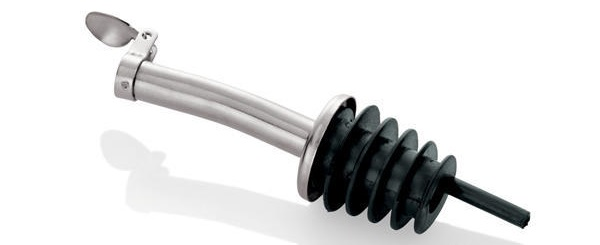
\includegraphics[scale=0.6]{obrazky/nalevac.jpg}
    \end{center}
    \label{nalevačos}
    \caption{Nalévátko na alkohol \cite{nalevatko}}
\end{figure}
% \definecolor{Silver}{rgb}{0.752,0.752,0.752}
% \begin{table}[!h]
%     \centering
%     \begin{tabular}
%         {
%         cell{1}{4} = {c},
%         hlines = {Silver},
%         vlines = {Silver},
%         }
%         Název & hmotnost\\
%         Nalévač č.1 & x\\
%     \end{tabular}
%     \caption{Caption}
%     \label{tab:my_label}
% \end{table}
%\usepackage{color}
%\usepackage{tabularray}
%\definecolor{Silver}{rgb}{0.752,0.752,0.752}
%\begin{tabular}[
%  label = none,
%  entry = none,
%]{
%  cell{1}{4} = {c},
%  hlines = {Silver},
%  vlines = {Silver},
%}
%Název destilátu & destilát č.1 & destilát č.2 & . . . \\
%EAN kód & & & \\
%hmotnost prázdné láhve & & & \\
%hmotnost plné láhve    &              & & \\
%hmotnost víčka         &              &              &       \\
%obrázek                &              &              &       \\
%max. objem             &              &              &       
%\end{tabular}
%Tabulka destilátů
%Nazev | EAN | k | q | m_víčko | max_objem | obrazek | poznamka
%Tabulka druhů nalévačů
%Nazev | m_nalevač | obrazek

\section{Váha}

Nejdůležitější komponentou systému je váha pro výpočet zbytkového objemu z naměřené hmotnosti láhve, viz kapitola č.\ref{Přepočet hmotnosti na objem}.  Proto v této podkapitole rozeberu požadavky, výběr váhy a její alternativy.
%
%Váhy jsou zařízení, která slouží k měření hmotnosti objektů. Existuje mnoho typů vah, ale základní princip je stejný. Váhy se skládají ze dvou hlavních částí: měřicího mechanismu a zobrazovacího mechanismu.
%
%Měřicí mechanismus se skládá z vážícího tělesa a pružiny. Když položíte objekt na váhu, pružina se stlačí a vážící těleso se posune dolů. Tento pohyb se přenáší na měřicí stupnici, která ukazuje hmotnost objektu.
%
%Zobrazovací mechanismus se skládá z displeje a elektronického obvodu. Elektronický obvod přijímá signál od měřicího mechanismu a převádí ho na čitelný formát pro displej. Displej pak zobrazuje hmotnost objektu.[zdroj]
%
%\subsection{Elektronická část váhy}
%
%Elektronická část váhy se skládá z senzoru a elektronického obvodu. Senzor měří deformaci, kterou způsobuje vážený objekt, a převádí ji na elektrický signál. Tento signál je poté zpracován elektronickým obvodem, který obsahuje A/D převodník a mikroprocesor.
%
%Senzory používané v elektronických vahách jsou obvykle tenzometry nebo load cells. Tenzometry jsou malé senzory, které měří změnu odporu, když jsou deformovány. Load cells jsou senzory, které měří změnu napětí, když jsou deformovány. Oba typy senzorů jsou velmi přesné a umožňují měření hmotnosti s vysokou přesností.
%
%A/D převodník převádí analogový signál z senzoru na digitální signál, který může být zpracován mikroprocesorem. Mikroprocesor pak zpracovává signál a zobrazuje výslednou hmotnost na displeji. [zdroj]
%
\subsection{Požadavky na váhu}

Hlavním požadavkem je oboustranný otevřený komunikační port pro čtení dat a odesílání požadavku na jejich zaslání prostřednictvím sériové linky do mikrokontroleru. (u kterého bude znám popis přenosu dat nebo-li data nebudou šifrována.) Tyto požadavky splňují většinou laboratorní a průmyslové váhy, kde se očekává, že data budou zpracovávána pomocí aplikace.

Váživost (maximální hmotnost, která lze na váze navážit) se požaduje minimálně 2 kg. Hmotnost prázdné láhve u většiny destilátů se pohybuje od 500 do 800 g a samotný obsah láhve je od 500 do 1000 ml, tudíž až necelý 1 kg. V případě robustnějších lahví okolo 1 kg by váživost do 2 kg nemusela stačit, proto je vhodnější volit 3 kg. Větší váživost jak 3 kg, by neměla pro běžné podniky HoReCa význam, navíc s vyšší váživostí úměrně klesá její přesnost a roste cena váhy.

Přesnost, jinak řečeno rozlišení nebo odčitatelnost, se udává v dílcích(d). Dílek je nejmenší hodnota hmotnosti, kterou lze z displeje váhy odečíst.\cite{vazivost} Měření zbytkového objemu destilátu při inventurách není záležitostí "laboratorního měření" a zákon nestanovuje s jakou přesností je nutné měřit objem v láhvích pro inventurní účely. Obecně na 
přesnost není kladen velký důraz. Tím, že žádná norma nestanovuje jakou přesnost by měl mít nově navržený měřicí systém, by bylo optimální, aby měřilo s přesností stejnou nebo vyšší než odměrné válce. Odměrné válce na alkohol (kapitola č. \ref{obecny_valec}) mají přesnost 40 ml. Obyčejné odměrné válce (kapitola č. \ref{valec_na_alkohol}) používané pro inventurní účely jsou běžně nižší třídy přesnosti, jako je třída B, kde přesnost měření není klíčová. Můžeme se setkat v gastro průmyslu i s odměrnými válci nejvyšší přesnosti a to s třídou A, které jsou primárně určeny pro laboratorní účely. Tyto válce dle normy ISO 4788, mají přesnost pro objem 1 litr: +-5 ml (celková přesnost 10 ml) a dělení stupnice po 10 ml. V praxi je přesnost měření menší ze tří důvodů:
\begin{enumerate}
    \item Skutečná chyba při měření nezávisí jen na přesnosti odměrného válce, ale také na schopnosti uživatele odhadnout hodnotu mezi dvěma ryskami.
    \item Přesnost se snižuje, pokud uživatel sleduje risku pod úhlem.
    \item Pokud uživatel měří objem při jiné teplotě než pro kterou je válec kalibrovaný (kapitola č.  \ref{Dosavadní metody měření - valce})
    %\item Odměrné válce jsou kalibrované pro měření při konkrétní teplotě, běžně se jedná o pokojovou teplotu 20 °C. V praxi se většina destilátů nachází v lednici, kde jsou chlazeny na 5 - 8 °C, což způsobuje menší objem naměřený na válci oproti skutečnému. Například, měří-li se při teplotě 5 °C destilát s vysokým obsahem alkoholu, např. 80\% z důvodu vyšší tepelné roztažnosti ethanolu oproti vodě, vyjde chyba 13,74 ml.
\end{enumerate}
Požadovaná přesnost váhy je rovna nebo menší jak 10 g (necelých 10 ml) v porovnání s odměrnými válci třídy A za předpokladu, že uživatel se vyhýbá třem výše zmíněným chybám.


Váha je určena pro fyzickou inventuru HoReCa podniků, která spadá pod interní činnost podniku a není podmínkou, aby byla certifikována viz. kapitola č.\ref{meridlo}
%Váha je určena pro interní chod podniku a není podmínkou, aby byla certifikována.

Po splnění výše zmíněných požadavků je rozhodujícím faktorem cena.
\\ \\
%zdroj: https://www.hepnar.cz/poradna/view/co-je-to-max-vazivost-a-dilek/
%Posledním parametrem je cena, kdy
%Váha by měla být kompaktní, aby ji bylo možné
%Při inventurách je hlavním problémem časová náročnost a 
%Přesnost v našem případě není až tak důležitou vlastností
\textbf{Souhrn požadavků prioritně seřazených:} %sestupně / 
\begin{itemize}
    \item Oboustranný otevřený komunikační port
    \item Váživost nad 2 kg
    \item Přesnost 10 g a více
    \item Nízká cena
\end{itemize}

\subsection{Vybraná váha}
%Při výběru váhy jsem se řídil výše zmíněnými požadavky, kdy. 

Váha byla vybrána na základě výše zmíněných požadavků.
Základní parametry váhy jsou vyobrazené v tab. č \ref{vahaa}.
%Kompletní dokumentace je v příloze č. x
Kompletní specifikace je uvedena v dokumentaci: \cite{vaha_datasheed}



\begin{table}[!h]
    \centering
    \begin{tabular}{|c|c|}
        \hline
        Výrobce                                                         & G\&G   \\ \hline
        Model                                                           & E3000  \\ \hline
        %\begin{tabular}[c]{@{}c@{}}Komunikační\\ protokol\end{tabular}  & UART   \\ \hline
        \begin{tabular}[c]{@{}c@{}}Komunikační \\ rozhraní\end{tabular} & RS-232 \\ \hline
        \begin{tabular}[c]{@{}c@{}}Datový \\ konektor\end{tabular} & \begin{tabular}[c]{@{}c@{}}DE-9\\ (Samice)\end{tabular} \\ \hline
        Váživost                                                        & 3 kg    \\ \hline
        Přesnost                                                        & 0.5 g     \\ \hline
        \begin{tabular}[c]{@{}c@{}}Doba \\ stabilizace\end{tabular} & < 2 s \\ \hline
        Cena                                                            & 1987 Kč     \\ \hline
    \end{tabular}
    \label{vahaa}
    \caption{Základní parametry vybrané váhy}
\end{table}

\begin{figure}[!h]
    \begin{center}
        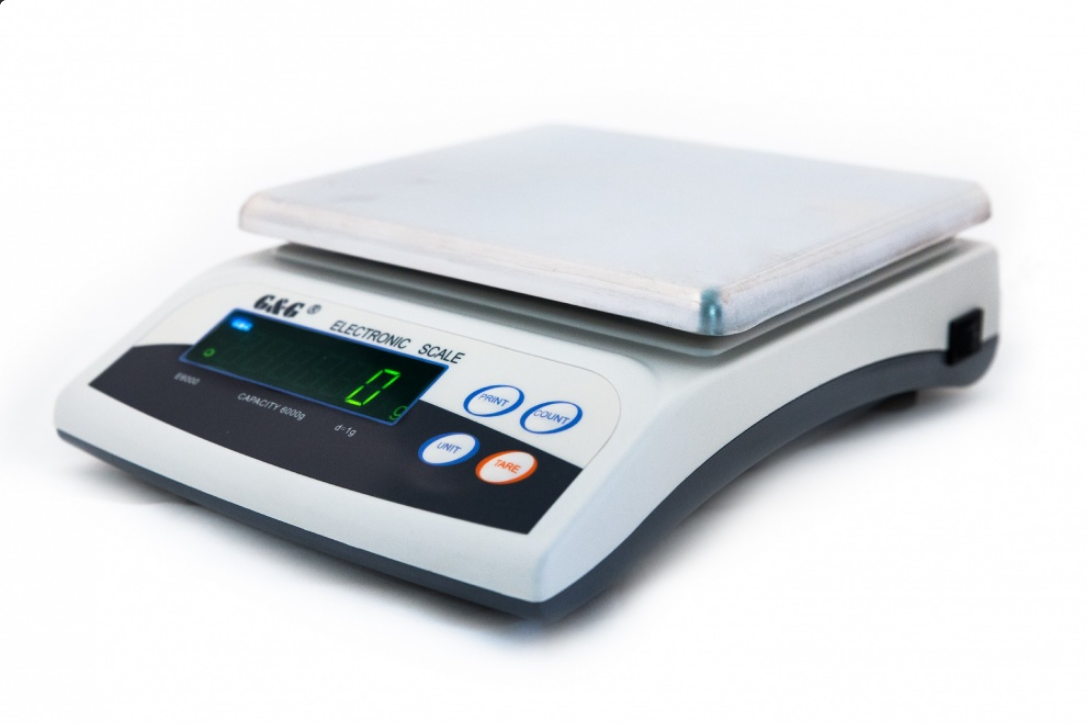
\includegraphics[scale=0.25]{obrazky/E3000.png}
    \end{center}
    \caption{Vybraná váha G\&G E3000 \cite{vaha}}
\end{figure}



% Jeden z hlavních požadavků bylo, aby váha obsahovala otevřený oboustranný komunikační port, jak pro čtení dat, tak i pro odesílání požadavků pro tisk.
% Zvolena váha disponuje RS-232 portem s komunikačním protokolem UART.

% Váživost byla volena 3Kg, protože většina větších destilátů váží do 2kg. Tudíž máme 1kg rezervu.

% Přesnost v našem případě nehraje, až tak významnou roli, proto byla váha vybírána na základě poměr "cena/výkon". Přesnost činní 0,5g.

%\subsection{Datový přenos}

%Váha posílá data přes RS-232 rozhraní. viz. kapitola č.x. Díky výstupnímu napětí 5V je možné bez nutnosti napěťového děliče připojit váhu přímo na vstup mikrokontroleru. Bohužel raspbery pi 4 disponuje pouze jedním UART rozhraním, který funguje v topologii pear-to-pear a bylo vyhrazeno pro senzor čárového kódu. Váha je tedy připojena na USB port, díky redukci RS-232 na USB, kdy propojení pinů je následovný:
%\begin{itemize}
%    \item Tx -> -D
%    \item Rx -> +D
%   \item COM -> COM
%\end{itemize}
%Napěťový vodič je pro náš systém zbytečný, proto není uvažován a datový vodiče jsou zapojený do kříže z důvodu pear-to-pear topologie.

\subsection{Datový paket}

Paket se skládá z:
\begin{itemize}
    \item 1 start bit
    \item 8 datových bitů
    \item 1 stop bit
    \item bez paritního bitu
\end{itemize}
V našem případě není vyžadován paritní bit z důvodu opětovného odesílání stejných dat na výstup. Přínos by mohl mít pokud bychom ukládali veškeré příchozí data. Systém vezneme pouze poslední příchozí hodnotu, pokud sekvence dat za touhle hodnotou byla neměnná(např. za ±1 sekundu), tedy že se nám ustálila naměřená hmotnost.

%\subsection{Datový rámec} %datový formát

%Datový rámec je část paketu, který obsahuje informace o hmotnosti viz. kapitola č.\ref{UARTt}. Dle dokumentace se formát skládá ze 14 bajtů zakódovaný v ASCII. Na obrázku č.\ref{data} je vidět posloupnost bajtů a jejich význam a na obrázku č.\ref{priklad} je praktický příklad.

%Datový rámec je část paketu, který obsahuje informace o hmotnosti viz. kapitola č.\ref{UARTt}. Dle dokumentace se formát skládá ze 14 bajtů zakódovaný v ASCII. Na obrázku č.\ref{data} je vidět posloupnost bajtů a jejich význam a na obrázku č.\ref{priklad} je praktický příklad.

Předpis výstupních dat se nachází v tabulce. \ref{tabos}, kdy dle dokumentace se formát skládá ze 14 bajtů zakódovaných v ASCII. V tabulce č. \ref{jouu} je praktický příklad.

%\begin{figure}[!h]
%    \begin{center}
%        \includegraphics[scale=0.5]{obrazky/data protokol - váha.PNG}
%    \end{center}
%    \label{data}
%    \caption{Předpis výstupních dat (1 unit = 1 bajt) \cite{vaha_datasheed}}
%\end{figure}

\begin{table} [!h]
    \centering
    \begin{tabular}{|l|l|l|l|l|l|}
    \hline
         Znaménko    & Mezera & Data &  Jednotka & Enter & Posun řádku \\ \hline
         1 B & 1 B           & 7 B           & 3 B &1 B&1 B\\ \hline
    \end{tabular}
    \caption{Předpis výstupních dat}
    \label{tabos}
\end{table}

%\begin{itemize}
%    \item space - "prázdný bit" %pro zachování velikosti 14-bitového slova
%    \item enter - přesunutí na začátek řádku (značení CR v ASCII: $\backslash$r)
%    \item linefeed - odřádkování (značeno LF, v ASCII: $\backslash$n) 
%\end{itemize}




\begin{table}[h]
\centering
\begin{tabular}{|p{0.6cm}|p{0.6cm}|p{0.6cm}|p{0.6cm}|p{0.6cm}|p{0.6cm}|p{0.6cm}|p{0.6cm}|p{0.6cm}|p{0.6cm}|p{0.6cm}|p{0.6cm}|p{0.6cm}|p{0.6cm}|}
\hline
\(\pm\) & SP & \multicolumn{7}{c|}{Data} & \multicolumn{3}{c|}{Jednotka} & CR & LF \\ \hline
- & \verb|␣| & \verb|␣| & 1 & 2 & 3 & . & 4 & 5 & \verb|␣| & g & \verb|␣| & \textbackslash{r} & \textbackslash{n} \\ \hline
\end{tabular}
%Pety navrhl
\caption{Příklad uspořádání dat v datovém formátu displeje}
%Můj navrh
%\caption{Příklad jak jsou data z displeje zapsány v datovém formátu}
\label{jouu}
\end{table}

\subsection{Alternativy vybrané váhy}
%Mezi alternativy k vybrané váze můžeme zařadit:
Níže je seznam s parametry vah dostupných na českém či zahraničním trhu jako alternativy k vybrané váze G\&G E3000. Váhy mají jako stejný parametr váživost 3 kg a oboustranný komunikační port RS-232, proto nejsou níže zmíněny.
\begin{itemize}
    %\item TRONIX ADX3B
    %\begin{itemize}
    %    %\item Váživost 3 kg
    %    \item Přesnost 0,1 g
    %    %\item Oboustraný komunikační port RS-232
    %    \item Cena: 2907 Kč
    %\end{itemize}
    
    \item G\&G E3KY05
    \begin{itemize}
        %\item Váživost 3 kg
        \item Přesnost 0,5 g
        %\item Oboustraný komunikační port RS-232
        \item Dokumentace je vysoce shodná jak u vybrané váhy G\&G E3000, proto je riziko, že by mohla být chybná
        \item Cena: 3935 Kč
    \end{itemize}
    
    \item U.S. Solid USS-DBS86
    \begin{itemize}
        %\item Váživost 3 kg
        \item Přesnost 0,1 g
        %\item Oboustraný komunikační port RS-232
        \item Cena: 1997,48 Kč
        \item Dostupná pouze v zahraničí
        \item Velice stručná dokumentace s chybějícími informacemi o komunikačním rozhraní
    \end{itemize}
    
    \item A\&D EK-3000i
    \begin{itemize}
        %\item Váživost 3 kg
        \item Přesnost 0,1 g
        %\item Oboustraný komunikační port RS-232
        \item Cena: 12670 Kč
        \item Obsáhlá dokumentace
        \item Certifikace
    \end{itemize} %G&G E3KY05 
\end{itemize}





%\begin{figure}[!h]
%    \begin{center}
%        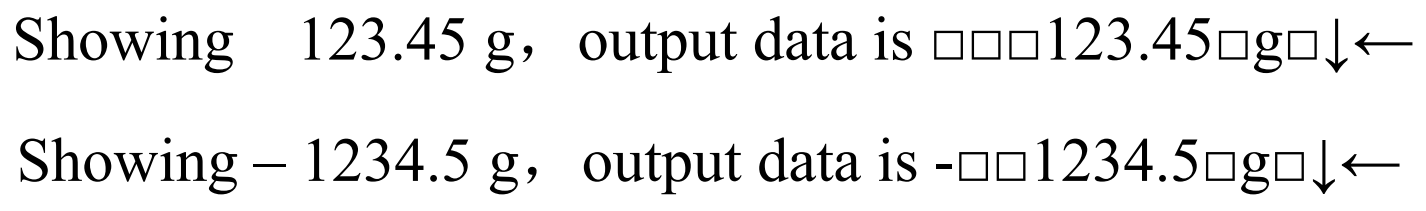
\includegraphics[scale=0.5]{obrazky/příklad protokolu - váha.PNG}
%    \end{center}
%    \label{priklad}
%    \caption{Příklad jak jsou data z displeje zapsány v datovém formátu \cite{vaha_datasheed}}
%\end{figure}



%Výstup reprezentovaný jako kod ASCII

%kombinace /r/n se vy uživa u WIndowsu k odřadkování pro 


%Vstupním portem je USB (viz. kapitola č. x), kdy piny

\section{Displej}
Další komponentou je displej, který je připojen k mikrokontroléru a zobrazuje název aktuálně měřeného destilátu, zůstatkový objem kapaliny v láhvi, maximální objem láhve, procento alkoholu měřeného destilátu a jeho obrázek pro případ, že by výrobce změnil tvar lahve, ale EAN kód by zůstal stejný.

\subsection{Požadavky na displej}
Hlavní požadavky na displej jsou:
\begin{itemize}
    \item Dotykový displej - pro budoucí implementaci klávesnice do displeje z důvodu redukce počtu periferií.
    \item Uhlopříčka 5 - 7 palců (12,7 - 17,78 cm) pro dobrou čitelnost
    \item Bez rámečků s montážními otvory - možnost displej uchytit k vlastnímu rámu 
\end{itemize}

\subsection{Výběr displeje}

Vybraný displej je JOY-IT RASPBERRY PI touch display 7". Jeho důležité parametry jsou v tabulce č. 5.4\\

\begin{table}[!h]
    \centering
    \begin{tabular}{|c|c|}
        \hline
        Výrobce                                                         & JOY-IT   \\ \hline
        Uhlopříčka                                                      & 7" (17,78 cm)  \\ \hline
        Rozlišení                                                        & 1024 × 600 px    \\ \hline
         Rozhraní 
            & HDMI, USB \\ \hline
        Dotykový displej                                                        & Ano     \\ \hline
        Cena                                                            & 2297 Kč     \\ \hline
    \end{tabular}
    \label{displeej}
    \caption{Základní parametry vybraného displeje}
\end{table}



\begin{figure}[!h]
    \begin{center}
        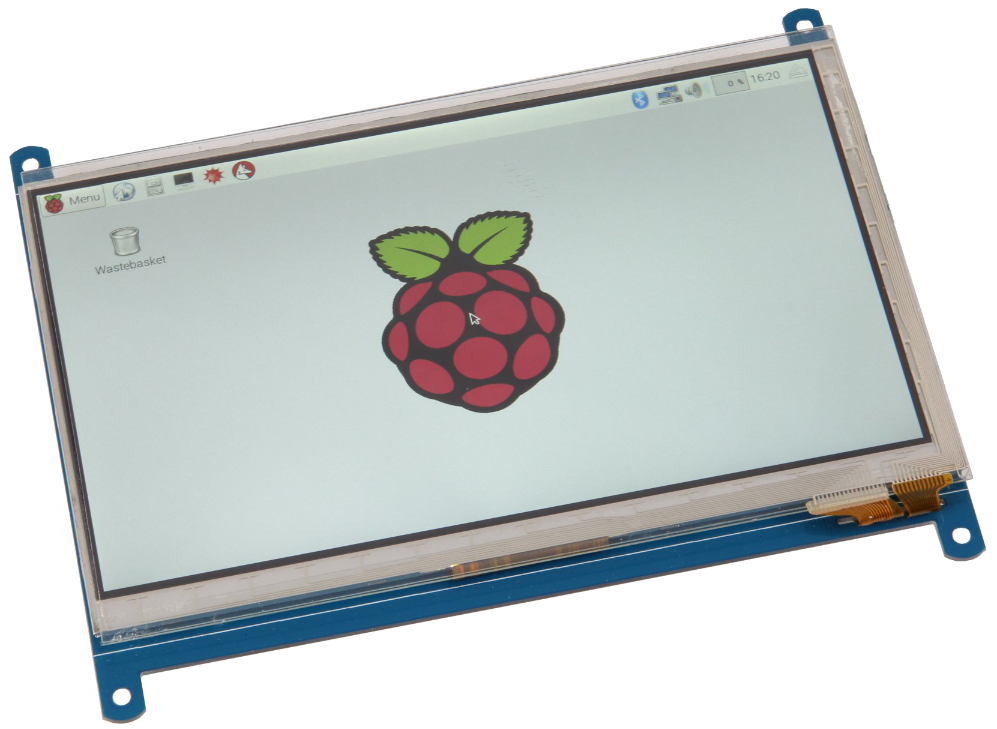
\includegraphics[scale=0.22]{obrazky/Displej.png}
    \end{center}
    \caption{Vybraný displej JOY-IT \cite{displej}}
\end{figure}

Mezi alternativy můžeme zařadit:
\begin{itemize}
    \item JOY-IT RASPBERRY PI touch display 5" - displej se liší od vybraného menší uhlopříčkou(5"), menším rozlišením(800x480) a nižší cenou(1599 Kč)
    \item Raspberry Pi LCD - 7" Touchscreen - displej se liší od vybraného menším rozlišením(800x480) a nižší cenou(1399 Kč). Jeho nevýhodou je horší dostupnost na českém trhu
\end{itemize}

%Displej je připojen k mikrokontroleru
%Displej nám bude zobrazovat data o 

\section{Čtečka čárového kódu}
Čtečka čárového kódu je zařízení, které jak jeho název napovídá, umí číst kód skládající se z černých proužků různých délek \cite{carovy_kod}, které reprezentují čísla splňující EAN standard.
%zdroj1: https://pageloot.com/cs/carovy-kod/jak-funguje-skener-carovych-kodu/
%zdroj2: https://cs.wikipedia.org/wiki/%C4%8Cte%C4%8Dka_%C4%8D%C3%A1rov%C3%A9ho_k%C3%B3du

EAN (European Article Number) je mezinárodní unikátní identifikační číslo, které usnadňuje prodejcům prodej zboží. Pro český trh se běžně využívá EAN-13 (13-ti místné číslo nacházející se nad čárovým kódem) \cite{EAN}
%zdroj: https://cs.wikipedia.org/wiki/European_Article_Number

%V praxi je toto číslo uloženo v databázi obchodu, které je spojeno s název produktu a jeho cenou. Po načtení čárového kódu. %Po načtení čárového kódu

V praxi je toto číslo uloženo v databázi obchodu, ke kterému je přiřazen název a cena produktu.

%Každé zboží se dá lehce indetifikovat pomocí

V této sekci se nebudeme zabývat, jakým způsobem jsou čísla kódována do této podoby, ale jakým způsobem lze tyto čárové kódy číst.

\subsection{Požadavky na čtečku čárového kódu}

Na trhu je dostupných více druhů senzorů, které se liší požadavky na přesnost, druh implementace, velikostí, atd.

Komunikační rozhraní čtečky se požaduje UART nebo USB s možností povolení virtuálního seriového portu pro komunikaci s mikrokontrolérem - označováno USB VCom.

Další požadavek spočívá v tom, aby čtečka byla schopna číst standard EAN-13, který je běžně používán v České republice, a také EAN-8, s nímž se lze výjimečně setkat.
\subsection{Vybraná čtečka čárového kódu}

Vybraná čtečka je GM65 od společnosti KROW, obrázek č.\ref{gm65}.
Čtečka disponuje UART a USB VCom. Kompletní specifikace je obsažena v dokumentaci.\cite{scaner}

\begin{figure}[!h]
    \begin{center}
        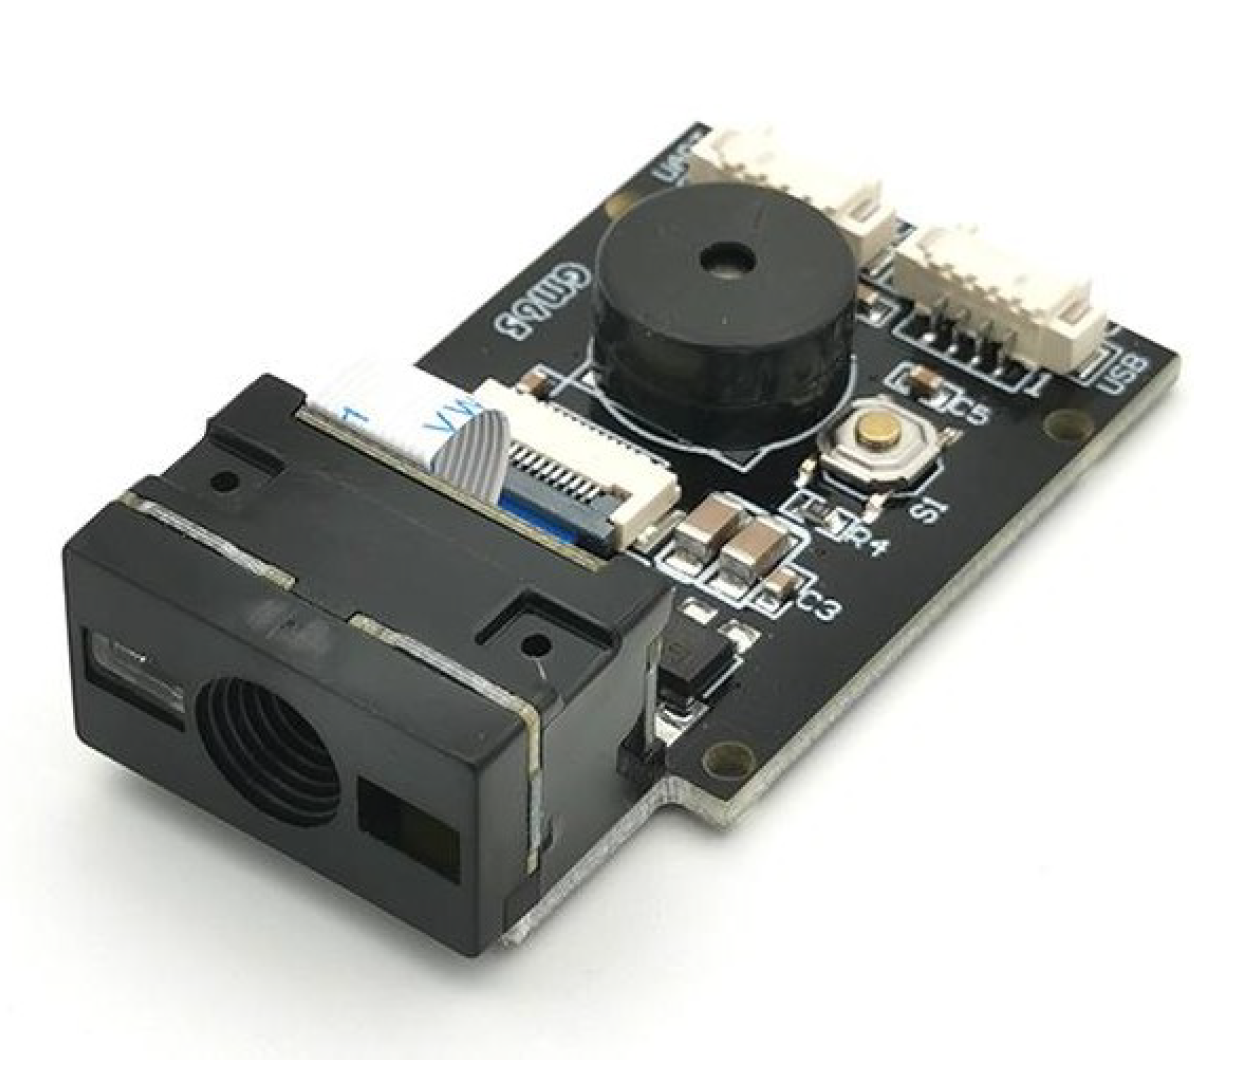
\includegraphics[scale=0.25]{obrazky/gm65.PNG} %0.5
    \end{center}
    \caption{Vybraná čtečka čárového kódu KROW GM65 \cite{scaner}}
    \label{gm65}
\end{figure}

Mezi alternativy můžeme zařadit:
\begin{itemize}
    \item YHDAA YHD-M800D - cenově stejně dostupné(1000 Kč) jak vybraná čtečka, integrovaný USB port, nepřehledná a nevypovídající dokumentace 
    \item WaveShare Barcode Scanner - dražší než vybraná čtečka(1318 Kč), integrovaný sériový port micro USB a UART
\end{itemize}

\section{Mikrokontrolér}

%Mikrokontroler jinak označovaný jednočipový počítač je integrovaný obvod
Mikrokontrolér nebo také jednočipový počítač je integrovaný obvod obsahující kompletní mikropočítač. Jednočipové počítače se vyznačují velkou spolehlivostí a kompaktností, proto jsou určeny především pro jednoúčelové aplikace. Mikrokontroléry jsou často používány v embedded systémech, jako jsou například řídicí systémy, regulátory, senzory a další aplikace, kde je potřeba rychle a spolehlivě zpracovávat data.%[zdroj]
%Na bakalařku překopat...je to opsaný
%https://sk.wikipedia.org/wiki/Mikrokontrol%C3%A9r
%https://cs.wikipedia.org/wiki/Jedno%C4%8Dipov%C3%BD_po%C4%8D%C3%ADta%C4%8D

\subsection{Požadavky na mikrokontrolér}
Hlavním z požadavků je snadná realizovatelnost firmware s integrovaným grafickým uživatelským rozhraním pro ovládání dotykového displeje. Pro takový účely je vhodné použít programovací jazyk Python, který nabízí široký výběr knihoven a nástrojů, které ulehčují a zrychlují vývoj samotného firmware.

Další z požadavků je 4x USB a 1x HDMI nebo Micro HDMI port pro připojení jednotlivých komponent měřicího systému - váha, EAN čtečka, displej a klávesnice.

Další požadavek je na integrovanou čtečku SD karty na které budou uložena veškerá data zmíněná v kapitole č. 5.3 o databázi.

Do budoucna je cílem bezdrátová konektivita s mikrokontrolérem pomocí mobilní aplikace nebo připojení se k ERP systémům, pro tyto účely požadujeme integrovaný Wi-Fi modul.

\subsection{Vybraný mikrokontrolér}
Na základě výše zmíněných požadavků byl vybrán ne mikrokontrolér, ale přímo jednodeskový počítač Raspberry Pi 4 4GB. Hlavní nevýhodou je pořizovací cena 1479 Kč a vyšší spotřeba energie v rozmezí 3 - 7 W. Kompletní specifikace se nachází v dokumentaci výrobce.[2] 

%Vybraný mikrokontroler byl Raspberry PI 4, který dokáže pokrýt veškeré požadavky na měřicí systém. Konkrétně se jedná o model B s 4 GB operační paměti. Zde jsou zmíněné požadavky na mikrokontrolér:

%\begin{itemize}
%    \item Dostatečný počet portů pro připojení všech modulů.
%    \item Integrovaná čtečka SD karty pro ukládání databáze
%    \item Dostatečný výkon pro chod GUI aplikací. Do budoucna je v plánu implementovat dotykový displej, na kterém budou veškeré informace pěkně přehledné díky grafickému rozhraní
%    \item Integrovaný čip pro bezdrátovou konektivitu. Do budoucna možnost vývoje mobilní aplikace k vyvíjenému systému nebo bezdrátové připojení k ERP systémům.
%    \item
%    \item Hlavní z požadavků je snadná realizovatelnost firmware s integrovaným grafickým uživatelským rozhraním pro ovládání dotykového displeje. Pro takový účely je vhodné použít programovací jazyk Python, který nabízí širší výběr knihoven a nástrojů, které ulehčují a zrychlují vývoj samotného firmware.
%
%    \item
%\end{itemize}
%Dost požadavků je nad rámec bakalářské práce, ale pro budoucí inovaci systému nemusíme měnit mikrokontrolér a realizovat znovu už fungující HW kompatibilitu mezi komponenty a vyvíjet SW vybavení.

%Jedinou nevýhodou je vysoká pořizovací cena.

\begin{figure}[!h]
    \begin{center}
        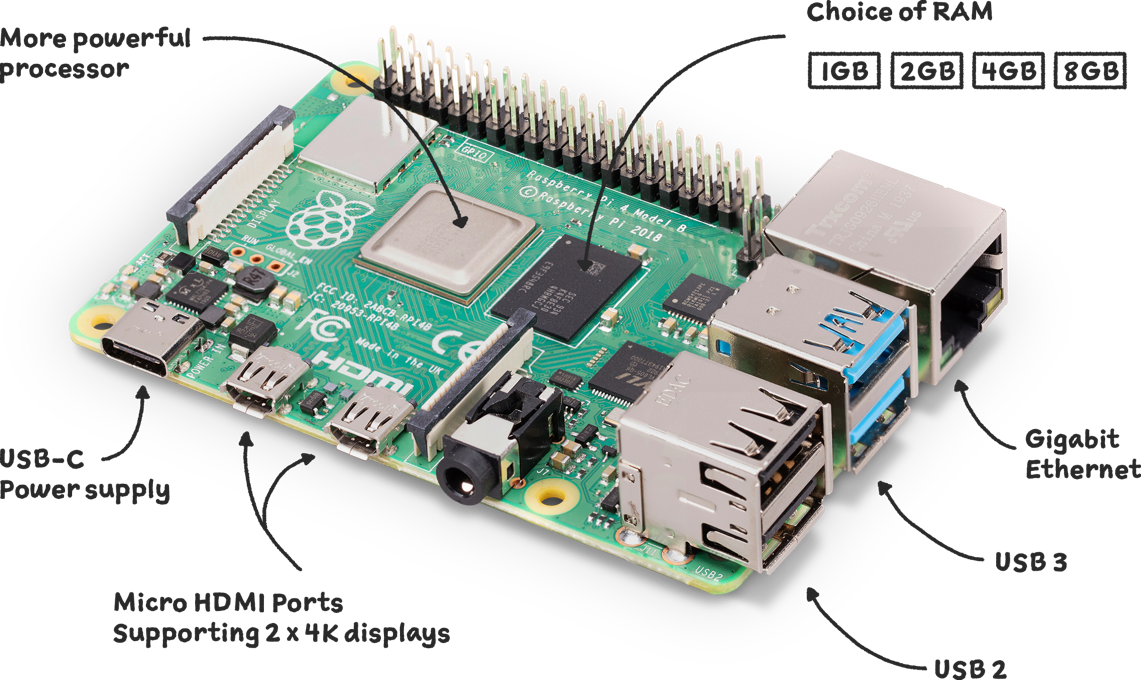
\includegraphics[scale=0.3]{obrazky/raspberry-pi-4.png}
    \end{center}
    \caption{Vybraný mikrokontrolér Raspberry Pi 4 \cite{malina_obr}}
    %\label{gm65}
\end{figure}

%Rozhodoval jsem se mezi dalšími dvoumi 







%proč malinu:
%
%-graficky čip pro dotykovy displej, 
%
%-wifi/BT čip pro budouci mobilni aplikaci, 
%
%-možnost vývoje GUI (python, CS) bezne mikrokontrole funguje jen na C/C++ asi,
%
%-rozumně velké uložiště pro ("GUI aplikaci" spíš RAM) databázi, která se časem bude rozšiřovat nevim jestli by arduino to pojmulo, ale určitě arduino nepojme databází obrázků, jednotlivých destilátů
%%https://www.dps-az.cz/clanky/id:6173/uvod-do-embedded-systemu